\section{Data}
\label{sec:data}

% \todo[inline]{Data: \textit{What kind of data are you going to use? If the data is available already: what are the key data characteristics?}}

% \todo[inline]{SemEval 2015 and/or SemEval 2016, and find source for document level data (He used Yelp2014 and Amazon Electronics dataset). Remove implicit data. Maybe some key characteristics are useful: Total count, Number of positives/negatives? Show whether the data is balanced or not, important for training an ML model}

The datasets used for ABSC are the SemEval 2015 \cite{SemEval2015} and SemEval 2016 data sets \cite{SemEval2016}. Specifically, our analysis focuses on restaurant reviews. Each review consists of one or more sentences, and each sentence contains the sentiment on one or more aspects. The sentiment can either be positive, neutral, or negative. In our research we focus on explicit aspects, which means that the aspect is present in the sentence. Figure \ref{fig:xml} shows an example sentence from the SemEval 2016 dataset in the XML markup language. This example shows that, in a review, multiple aspects can be present and the sentiment towards different aspects may differ. Table \ref{describeData} gives the descriptive statistics of the SemEval 2015 and the SemEval 2016 data sets. One can notice that there are relatively few neutral reviews. Furthermore, in most data the positive class is the majority class, except for the test data of the SemEval 2015 data set. The 2015 dataset is noticably smaller than the one from 2016.


\begin{figure}
    \centering
    \frame{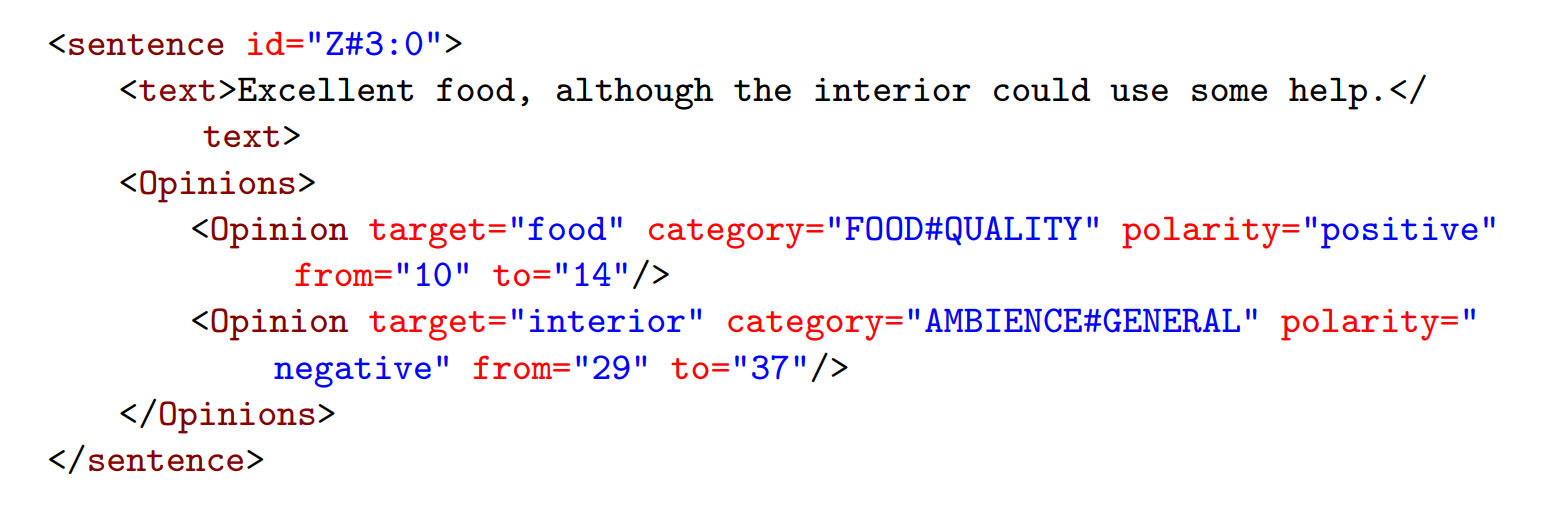
\includegraphics[scale = 0.4]{Images/xml code.PNG}}
    \caption{A sentence from the SemEval 2016 dataset.}
    \label{fig:xml}
\end{figure}


We use a document-level dataset from Yelp2014 \cite{Tang2016} for pretraining, as it matches the domain of our aspect-level data: restaurants. However, these reviews are classified on a 5-point scale. Therefore, the reviews will be labeled in the following way: reviews with ratings $>3$, $=3$, and $<3$ are labeled as positive, neutral, and negative, respectively. Similar to \cite{He2018}, a balanced sample of 30000 will be extracted from the dataset to obtain our pretraining corpus. As Table \ref{describeData} shows, there is a significant lack of neutral examples in the aspect-level data. Therefore, the balancing of the pretraining corpus allows the model to see an ample amount of documents for each category. To make our data suitable for multi-task learning, each aspect-level datapoint is paired with a random document from our sample. As there are many more documents available than aspects, we upsample our aspect-level data with a factor of three. This value was chosen from intuition, as too little upsampling will not allow us to exploit many documents whereas too much upsampling will likely lead the model to overfit due to the duplicates in the aspect data.

\begin{table}[h]
\caption{Descriptive statistics of the SemEval 2015 and semEval 2016 datasets, split into training and test data.}
\label{describeData}
\setlength{\tabcolsep}{8.2pt}
\begin{tabular}{@{}lccccccc@{}}
\toprule
\multicolumn{1}{c}{\multirow{2}{*}{Dataset}} & \multicolumn{2}{c}{Positive} & \multicolumn{2}{c}{Neutral} & \multicolumn{2}{c}{Negative} & Total \\ \cmidrule(l){2-8} 
\multicolumn{1}{c}{}                         & Freq          & \%           & Freq          & \%          & Freq          & \%           & Freq  \\ \midrule
SemEval-2015 training data                   & 963           & 75.3         & 36            & 2.8         & 280           & 21.9         & 1279  \\
SemEval-2015 test data                       & 208           & 34.7         & 38            & 6.3         & 354           & 59.0         & 600   \\
SemEval-2016 training data                   & 1321          & 70.1         & 73            & 3.9         & 490           & 26.0         & 1884  \\
SemEval-2016 test data                       & 487           & 74.4         & 32            & 4.9         & 136           & 20.8         & 655   \\ \bottomrule
\end{tabular}
\vspace{-5mm}
\end{table}
